\begin{wrapfigure}[18]{r}{8cm}
  \centering
  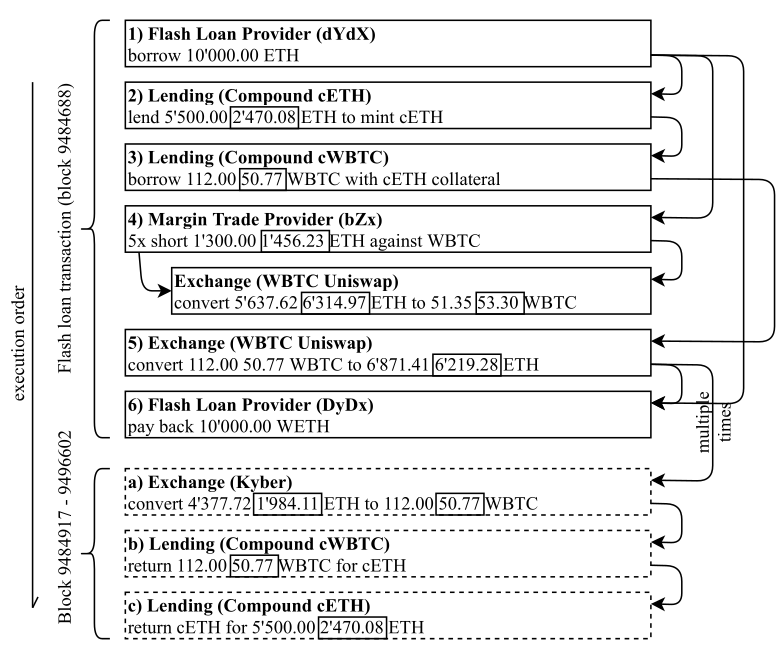
\includegraphics[width=8cm]{assests/pump-and-arb}
  \caption{Caption}
  \label{fig:pumpAndArb}
\end{wrapfigure}
\paragraph{Pump and arbitrage} A visualization of this example can be see in figure \ref{fig:pumpAndArb}, figure \ref{fig:pumpAndArb} is from \cite{attack} where they describe the procedure, which we will explain here.

The main part of this trade is a margin trade on the DEX bZx to increase the price on the Uniswap DEX. The trader uses this manipulated price on Uniswap for arbitrage. Let look at exactly what the trader does, by looking at figure \ref{fig:pumpAndArb}; 1) A flash loan is taken with the trader borrowing 10,000 ETH 2) he then lends 5,500 ETH to mint 274,843.68 cETH 3) which he uses as collateral to borrow 112.00 WBTC. 4) He then performs a margin trade, with 5x leverage, for ETH against WBTC on bZx. When bZx receives the request they convert 5,637.62 ETH to 51.35 WBTC, that is 109.79 ETH/WBTC on average with a high of 124.41 ETH/WBTC, for context, at the start of the block this transaction happened in Uniswap was at 36.55 ETH/WBTC, this means that the price slipped from 36.55 to 124.41 that is a slippage of $\frac{124.41-36.55}{36.55}\approx 240\%$ which both Uniswap\footnote{This is with Uniswap v1} and bZx allows. 5) The trader then converts the 112.00 WBTC he borrowed earlier, to 6,871.41 ETH (at 61.35 ETH/WBTC). 6) The trader then pays back the loan with the remaining 3200 ETH from the flash loan and the 6,871.41 ETH he just got, netting a profit off 71.41 ETH, however this is not the real price, the real price is the over-collateralized loan of 5,500 ETH for 112 WBTC at 49.10 ETH/WBTC because this is fairly high so over a period of two days (steps a-c in figure \ref{pumpAndArb}) the trader exchanges 4,377.72 ETH for 112 WBTC, at 39.08 ETH/WBTC, to redeem the 5,500 ETH thereby making 10.02 ETH per WBTC and adding in the 71.41 he made earlier the total profit is 1,193.65 ETH.

\begin{wrapfigure}[18]{r}{8cm}
  \centering
  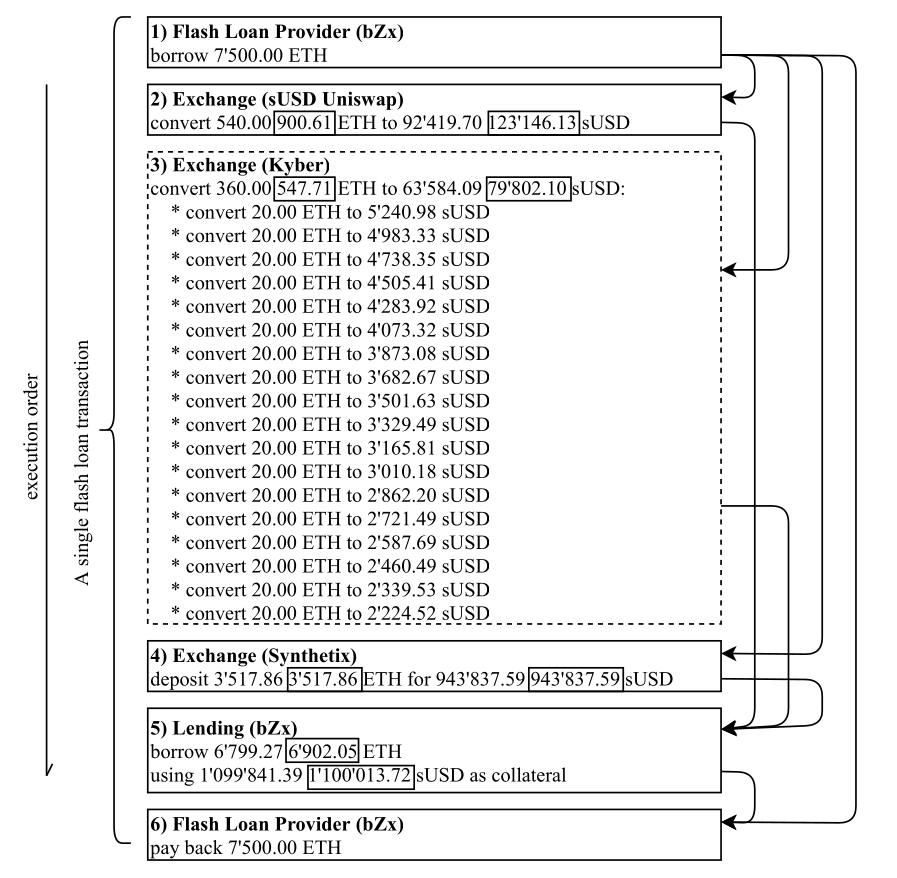
\includegraphics[width=8cm]{assests/oracle}
  \caption{Caption}
  \label{fig:oracle}
\end{wrapfigure}
\paragraph{Oracle manipulation} A visualization of this example can be see in figure \ref{fig:oracle}, figure \ref{fig:oracle} is from \cite{attack} where they describe the procedure, which we will explain here.

The main part of this trade is converting ETH to sUSD to in order to lower the price of sUSD/ETH, and then lend from a platform who uses the conversion rate to borrow ETH at a low cost. In more detail the trader; 1) borrows 7,500 ETH using a flash loan 2) convert 540 ETH to 92,419.7 sUDS at 171.15 sUSD/ETH (on the Kyber-Uniswap reserve), 3) he then converts 360 ETH to 63,584.09 sUSD at 111.23 sUSD/ETH (on Kyber)